\chapter{基于统计的错误定位}
\label{cha:fl}

\section{引言}
\label{sec: introduction}
错误定位是“生成-检验”框架的第一个工作步骤,基于统计的错误定位(Spectrum-based Fault Localization,简称SFL)算法因其实现简单、效果良好被绝大多数现有系统采用。SFL的基本思想是,利用“被通过的测试用例执行次数越多的语句越可能是正确的,被不通过的测试用例执行次数越少的语句越可能是错误的”这一经验规律,通过统计各个程序语句在各个测试用例中的执行次数,按照某一公式计算各个语句出错的可能性,并将语句按此排序,最终开发人员可以按照此排序逐一检查程序语句。实践表明,通常真正错误的语句会被排在非常靠前的位置,因此开发人员能够省去查看其它正确语句的时间。

SFL计算结果的合理性依赖软件工程中一项称为“测试准则假设(Test Oracle Assumption)”的基本假设,其内容是在测试过程中,总存在一种判断机制,或者称作测试准则(Test Oracle),能够准确的判断被测程序是否正确的执行了一条测试用例\cite{Peters:1994:GTO:186258.186508}。该假设被广泛接受,已经成为许多软件工程问题的分析基础。然而在实际开发过程中,完全正确的测试准则是很难获得的。面对越来越复杂的软件系统,现有的测试准则的自动生成技术远远无法满足需求 \cite{harman2013comprehensive}。事实上,对测试结果进行人工检查仍然是工业界广泛采用的工作方法\cite{manolache2001software}。换言之,人工判断成为了实际应用中的“测试准则”。

使用人工检查作为测试准则会引发严重的问题。人工检查很容易出错\cite{manolache2001software},因此我们所承认和依赖的“测试准则假设”不复存在,测试人员实际上并不能够完全正确的判断被测程序是否真的通过了一个测试用例。这种判断错误在许多情况下都可能出现。例如,对于复杂的软件系统,测试人员很可能无法对程序的所有部分都有清晰准确的理解和认识,因此判断一个具体的测试结果也有一定的难度。另外,当程序的行为比较复杂时,通常需要一个非常大的测试集,由于测试用例基数大,判断失误不可避免。在文章~\cite{mcminn2010reducing}中作者提到,当测试用例的输入是由一些测试用例生成工具产生时,工具所生成处的测试输入可能比较抽象(如无意义的字符串),测试人员难以直观理解,这也为判断测试结果的正确性带来了难度。以上这些场景在实际开发过程中非常常见,因此开发人员在日常工作中所使用的测试准则往往是有错的。

SFL计算公式中的输入数据直接来自测试准则判断结果,因此测试准则错误将使SFL计算结果精度下降。事实上,由本章第3节中的实验数据可见,精度越高的SFL公式对准则错误越敏感。因此,若要使SFL在“生成-检验”系统中发挥作用,则需要尽量消除测试准则错误对SFL带来的负面影响。

想要消除这一负面影响的一种直接的办法是,抛弃原有的测试准则并重建一套新的测试准则。然而,新的测试准则可能并不比上一套正确率更高,而重建也需要耗费大量的时间和资源。再者,原有的测试准则虽然含有一定的错误,但是其中绝大多数的判断仍是正确的,具有利用价值。因此一个更好的思路是设计一种算法,能够直接改正在原有测试准则上的错误。在本章中,我们提出一种测试准则的自动化纠错技术,它能够发现测试准则做出的错误判断,使得SFL计算结果尽量不受影响。

本章提出的测试准则自动化纠错技术是是基于以下观察:通过相似测试路径的测试用例通常具有相同的测试结果(通过、不通过)。这一观察实际来源于基于覆盖率的测试集压缩技术\cite{wong1995effect}\cite{wong1999test}。我们试图给出测试用例之间相似度的度量方法,并识别出与其近邻测试结果明显不同的测试用例,将其标为“疑似错误”,并在SFL的输入中将其测试结果取反(及将“通过”改为“不通过”,反之亦然)。这一处理过程计算简单,但实验证明效果良好。

为全面评价这一技术,我们采用了软件基础设施库(Software Infrastructure Repository\cite{doESE05})中的两组实际程序作为测试对象,第一组是西门子测试集(Siemens Test Suites),它被错误定位算法设计研究工作广泛采用。
第二组是\texttt{grep} 是Unix系统下的实际程序,其代码规模达到13,000行。我们首先为西门子测试集中的7个测试程序的132个变体生成了错误率在0.01-0.1之间的测试准则(即测试准则判断测试结果出错的概率在0.01-0.1之间)。同时我们也为4个版本的\texttt{grep}程序生成了相同错误率的测试准则。实验表明,经过自动化纠错处理,所识别出的“疑似错误”测试结果有75\%是真正的测试准则错误。此外,将SFL应用于被纠正后的测试结果时,几种SFL算法的精确度相较使用未纠错的测试结果均有了较大幅度的提高。

本章的主要贡献包括:
\begin{itemize}
	\item 在西门子测试集上,以实验证明测试准则的错误将有损SFL技术的错误定位准确度。这是目前已知第一项在测试准则出错前提下分析SFL技术精度的研究工作。
	\item 提出一项简单而有效的自动化测试准则纠错算法。实验表明,该算法能够识别出测试结果判断错误中的75\%,而经过纠错的测试结果也使得SFL算法精度大幅恢复。
	\item 定量分析不同类型的测试准则判断错误(如“假通过”和“假失败”)对SFL精度的影响。
\end{itemize}

本章余下内容的组织结构如下:第二节总结相关工作,第三节以实验数据阐明测试准则纠错的必要性,第四节介绍测试准则纠错算法,第五节展示算法的实际效果,并对实验结果进行深入分析,第六节总结本章工作。

\section{相关工作}
本章工作的核心内容是测试准则纠错算法,至今这是第一项探究测试准则错误与SFL精确度之间关系的研究工作。与之联系紧密的研究内容可分为如下三类:(1)对各个SFL算法精确度的测评,(2)分析与SFL算法精度相关的因素及其对SFL的影响,(3)测试准则自动生成技术研究。以下将按类别逐一介绍这些研究内容。

\subsection{SFL算法精度测评}

测评SFL精度的工作已有很多,包括实验分析和理论分析两类。
\cite{Jones:2005:EET:1101908.1101949}将Tarantula算法与之前的错误定位算法如Set union, Set intersection, Nearest neighbour和Cause transitions在测试集上的实验结果进行对比分析。作者得出的结论是Tarantula在诸多算法中取得了最好的效果。\cite{4041886}对四种SFL算法中用到的计算公式进行测试,得出结论是Ochiai在所有被测程序中一致的优于Jaccard和Tarantula,Jaccard不弱于Tarantula,而AMPLE的精度与其他公式相比时优时劣。 以上两篇工作都以Siemens Test Suite作为目标程序。更进一步,\cite{Abreu20091780}将Ochiai, Tarantula,Jaccard和其他6个计算公式在Siemens Test Suite和\texttt{space}程序上做对比测试实验,数据显示Ochiai精确度最高。Naish et al. \cite{Naish:2011:MSS:2000791.2000795} 对41种计算公式进行理论分析,最终将其按精确度划分为6组,其中每组内公式在单一错误前提,即程序中只有一个错误的前提下理论上都是等价的。Xie et al.\cite{xie2013theoretical}分析了30条计算公式并将其按精确度划分为14个等价类。该研究进一步分析了在单一错误前提下几个等价类之间的优劣关系,证明了两组公式ER1 (包括Naish1, Naish2两个公式)和ER5 (包括Binary, Russel\&Rao, Wong1三个公式)是理论上的最优公式。
在此结论基础上\cite{6676912}对Tarantula,Ochiai以及ER1和ER5中的公式进行了实际实验。实验结果表明,Ochiai的实测精确度比ER1和ER5两组高,而Tarantula的精确度平均值也优于ER1中的Naishi1和ER5中的全部算式。这与\cite{xie2013theoretical}中的理论分析矛盾,作者分析可能的原因是理论分析中假设代码覆盖率为100\%,而实际程序中覆盖率达不到这一数值。本文\ref{subsection: compr result}节中对几个SFL计算公式的测试数据考虑了测试准则出错的可能性,为以上工作做了补充。
\subsection{影响SFL精确度的因素}

研究表明,SFL算法的精度受许多因素的影响,对这些影响进行定性或定量的分析也是SFL算法的研究内容之一。在~\cite{Abreu20091780},作者研究了测试用例总数、通过的测试用例数与未通过的测试用例数对SFL精度的影响。分析结果表明,想要获得接近最优的精确度,即将真正错误的代码行排在前20\%仅需有限的测试集规模就可达到。在~\cite{Yu:2008:ESE:1368088.1368116}中,作者研究了使用10种测试集压缩策略缩减测试集对SFL精确度的影响。研究表明,SFL算法的有效性确实会受到测试集压缩策略的影响。
\cite{Masri:2009:ESF:1555860.1555862}讨论了四种与测试或测试集相关的场景,并首次提出了两个概念:(1)“巧合通过”(Coincidental correctness),意指在一次测试中程序出错条件已经触发,但是实际执行过程中测试却并没有失败的情形,(2)“弱巧合通过”(Weak coincidental correctness),指出错的语句被执行到,但测试结果最终并没有出错的情况。基于以上观察,后来的研究者提出使用测试聚类\cite{5477086}\cite{Masri:2014:PCC:2582050.2559932}和基于上下文模式的覆盖率精化方法\cite{Wang:2009:TCC:1555001.1555022}消除这两种情况对SFL精度的影响。注意,这里的“(弱)巧合通过”是测试准则的正确判断,与本章工作中关注的测试准则错误并不相同。
\cite{Kochhar:2014:BFM:2597073.2597105}\cite{Herzig:2013:IBI:2486788.2486840}注意到软件开发过程中产生的错误报告会被分到错误的类别中,这种分类错误也会对错误定位和预测产生影响。这与本章工作的相同点在于,他们并不假定人工提交的错误报告在人工判断类别时完全正确,但是这两篇工作关注的错误定位粒度在文件级,而非代码级。

\subsection{测试准则的自动生成}

在软件测试过程中,测试准则是判断程序是否运行正确的唯一标准。然而,自动生成可靠的测试准则并不简单。尽管以人工判断作为测试准则仍然常见于工业界,现在已有越来越多的研究工作尝试自动生成可靠的测试准则,节省开发时间。

测试准则的自动生成方法可划分为两类。第一类是生成显式的测试准则。例如,在\cite{Memon:2000:ATO:357474.355050}中,作者提出了一种自动判断GUI操作响应正确性的方法。被测GUI程序首先被建模为一组对象的集合,同时每个对象的属性和动作及对动作的反应都被形式化的描述。在执行测试程序时,系统可以自动的判断程序的实际行为是否满足之前的形式化描述。尽管最后的系统判断是完全自动的,系统仍然依赖开始时对GUI程序的形式化描述,并且由于GUI程序的特殊性,这一技术很难扩展到其他类型的程序中。
在\cite{Aggarwal:2004:NNB:986710.986725}, 作者研究了将人工神经网络( Artificial Neural Networks,缩写为ANN)用作三角形分类问题的测试准则的正确率。作者最终得出的结论是,ANN的判断出错概率约为19.02\%,而这一准确率达到了实用的要求。然而在本章第5节的实验数据显示,准确率仅为80.98\%的测试准则在实际应用中会给程序调试带来严重的影响。将这一方法推广到其他程序也具有一定的困难。
另一种有趣的思路是从软件文档中直接生成测试准则\cite{667877-documentation}。然而,使用这种方法的前提是软件文档按照文中定义的书写规范精确地定义了软件系统的行为,因此对于已经开发很长时间的遗留系统很难适用。

第二类工作避免了显示地生成一组测试准则,而以其他策略判断被测程序的测试结果。在\cite{Davis:1981:PNP:800175.809889}中, Davis et al.首先提出对不容易测试的程序可独立开发满足同一设计规约的多个版本程序作为“假测试准则(pseudo oracles)"。作者建议使用两个或多个版本的程序运行同样的测试用例,当测试输出不相同时,可使用某种投票机制决定哪个结果是正确的。显然,与第一类策略相比,使用这种策略将引入大量的编码工作。一个改进的策略发表于\cite{257793-1992},作者提出其他独立版本的程序可以使用代码自动生成技术来开发,而此时
引入的额外工作仅仅是对程序行为进行形式化的描述。这显然是上一工作的重要改进,可惜的是并非所有的程序都适合用形式化规约来描述其行为,因此其适用范围也比较有限。
在测试准则不易获取的情况下,蜕变测试(Metamorphic testing)也是常用的测试方法。蜕变测试不依赖形式规约,它的基本思想是将程序按某种规则变换后判断其输出结果的变化是否符合预期。在\cite{960614-chen-2001}和\cite{Chen20031}中,作者提出可以将蜕变测试与使用符号输入的基于错误的测试方法相结合%TODO:
,但没有阐述具体的系统实现及其实验效果。接下来,\cite{murphy2010automatic}\cite{Murphy:2009:AST:1572272.1572295}推出了工具Amsterdam,它可以自动化蜕变测试过程。 遗憾的是,尽管测试过程可以自动化执行,测试人员仍然需要人工描述蜕变测试中程序所应满足的属性,例如输入应如何变形,而输出应具有怎样的变化。在\cite{cheon2005complete}中,作者声称测试过程已经完全自动化了,其中包括测试准则的自动化生成。而事实上,测试准则仍然存在,只是转化为了使用Java建模语言(Java Modeling Language,简称JML)描述的断言(Assertions)、前置和后置条件(Pre- and Post-conditions)及类不变量(Class Invariants)。严格来讲,这些工作仍然是人工完成的,因此测试过程并不能够称为“完全自动化的”。


总之,自动生成测试准则技术尚未成熟,这也是本章工作的主要动机之一。在我们尚不能够完全自动的生成测试准则时,应当尽量充分的利用不完善的测试准则库,使其能够对错误定位和修复产生正面作用。

\section{测试Oracle纠错的必要性}
\label{sec: error impact}
%This is the illustrative example
%\begin{landscape}

\begin{table}[!t]
	\centering
	\caption{Debugging Process of a Sorting Program}\label{tab: Sorting}
	\begin{tabular}{l|c|c|c|c|c|c|c|c}
		\hline Input: (a, b, c) & $(1,2,3)$ & $(1,3,2)$ & $(2,1,3)$ & $(2,3,1)$ & $(3,1,2)$ & $(3,2,1)$ & $Sus_c$ & $Sus_e$ \\ 
		\hline 1\ \texttt{if(a>b)\{} & \textbullet & \textbullet & \textbullet & \textbullet & \textbullet & \textbullet & $0.5$ & $0.5$ \\ 
		\cline{2-9} 2\ \ \ \texttt{swap(a,b);} &  &  & \textbullet &  & \textbullet & \textbullet & $0.5$ & $1.0$ \\ 
		\cline{2-9} 3\ \texttt{if(b>c)\{} & \textbullet & \textbullet & \textbullet & \textbullet & \textbullet & \textbullet & $0.5$ & $0.5$ \\ 
		\cline{2-9} 4\ \ \ \texttt{swap(b,c);} & \textbullet &  &  & \textbullet & \textbullet & \textbullet & $1.0$ & $0.6$ \\ 
		\cline{2-9} 5\ \ \ \texttt{\color{red}if(a<b)} & \textbullet &  &  & \textbullet & \textbullet & \textbullet & $1.0$ & $0.6$ \\ 
		\cline{2-9} 6\ \ \ \ \ \texttt{swap(a,b);} & \textbullet &  &  &  & \textbullet &  & $1.0$ & $0.3$ \\ 
		\cline{2-9} 7\ \texttt{\}} &  &  &  &  &  &  & $-$ & $-$ \\ 
		
		\hline Oracle(correct) & $\times$ & $\checkmark$ & $\checkmark$ & $\times$ & $\times$ & $\times$ &  &  \\ 
		\hline Oracle(error) & \color{red}$\checkmark$ & $\checkmark$ & \color{red}$\times$ & $\times$ & $\times$ & $\times$ &  &  \\ 
		\hline 
	\end{tabular} 
\end{table}
%\end{landscape}
测试准则错误指的是对测试结果的一项错误的判断,例如程序在运行某一测试时实际执行正确,但测试准则却判定其执行错误,测试不通过,或者相反。这种情况会可能会令开发人员非常费解,不可避免的花费许多时间理清其中的问题,例如需要跟踪程序的执行过程,查看、确认是被测代码的问题还是测试代码的错误。如果使用自动错误定位算法,算法的准确度也受到影响,使得开发人员无法充分利用这些技术带来的便利。下一小结的例程对这一情况将有更好的解释。

\subsection{例程}
表\ref{tab: Sorting}展示了一个简单的排序程序及其配套的一组测试用例。程序的目的是将输入的三个数值变量a,b,c按照从小到大的顺序排序。开发人员在程序的第5行(标红)不小心写错了if条件判断表达式,本应是判断(a>b)但实际程序中比较符号方向写反了。这一组测试用例包含六组输入数据,分别覆盖了常见的六种变量间的大小关系。我们将六组测试用例对程序语句的覆盖情况用点号和空格标识,例如第一组数据覆盖了程序的第1行和3~6行,则在这项行号上标识点号。表格的最后两行给出了两组测试准则对各个测试用例通过与否的判断,打钩表示通过,叉号表示不通过。第一组对测试通过与否判断正确,而第二组对第1组和第3组测试的判断错误(标红)。

在调试过程中,开发人员可以借助自动错误定位技术的帮助来节省调试时间。自动错误定位技术将代码行按照出错的可能性进行排序,开发人员可依照这个排序列表逐一检查代码行,省去查看不太可能出错的位置花费的时间。基于频谱的错误定位(Spectrum-based Fault Localization,简称SFL)是一类轻量级的错误定位算法。其输入是测试用例的执行路径(称为频谱)以及测试结果(称为诊断)。据此,SFL对每一行代码$c$统计以下四项数据,覆盖$c$且通过的测试用例数$a_{ep}$,覆盖$c$且未通过的测试用例数$a_{ef}$,未覆盖$c$且通过的测试用例数$a_{np}$及未覆盖$c$且未通过的测试用例数$a_{nf}$。根据这些统计数据,SFL使用一条计算公式估计代码行$c$的“可疑程度”,即其是错误代码行的可能性。最终,可疑程度高的代码行被排在靠前的位置。

例如,知名的SFL算法Tarantula\cite{jones2002visualization}的计算公式如下:
$$
\frac{\frac{a_{ef}}{a_{ef} + a_{nf}}}{\frac{a_{ef}}{a_{ef} + a_{nf}} + \frac{a_{ep}}{a_{ep} + a_{np}}}
$$
Tarantula的基本思想很简单:对于任意一行代码$c$,覆盖$c$且失败的测试用例比例越高,$c$越有可能是错误的代码行。在表\ref{tab: Sorting}的例子中,我们将Tarantula依据正确和错误的测试准则判断计算出的可疑程度值分列在表格的最后两列。当使用正确的测试准则时,Tarantula指出具有最高可疑值的代码行是第4,5,6三行。假设开发人员完全依照这一排序进行检查,那么他应该随机的按任意顺序检查这三行,平均来看他将在检查第二个代码行时检查到第5行并发现错误。但是如果使用错误的测试准则,Tarantula会将第2行排在最靠前的位置,于是开发人员在检查第4行和第5行前需要先检查第2行。于是,平均来看他将在检查第2.5个代码行时遇到第5行并发现错误。

由上例可以看出,Tarantula的性能由于测试准则的错误受损。尽管多检查$0.5$行看起来并不是非常严重的性能损耗,但是这只是一个7行的小程序。由下一小节的实验数据可以看出,由于测试准则出错带来的性能损耗百分比实际上与程序规模关系不大。对较大规模的程序,这些损耗将使得系统的整体效率明显降低。

\subsection{在西门子测试集上的实验}

为了对测试准则带来的定位精度损耗有更清晰的认识,我们在西门子测试集(Siemens Test Suites)上进行了实验。西门子测试集包括7个不同的程序以及他们的变体共132个。有关该测试集在\ref{subsection data collection}小节有更详细的数据介绍。在此测试集上,我们选取了4种具有代表性的SFL算法,分别统计它们在正确和错误的测试准则下的定位精确度并加以比较,分析其精度受损程度与测试准则错误率之间的关系。

\subsubsection{定义SFL的算法精度}

为后续的清晰讨论,本节我们给出SFL算法定位精度的详细定义。当被测程序只有一个错误时,定位精度可以被自然地定义为在检查到真正错误的代码行之前所需检查的代码占所有代码行总数的比例。但是实际程序中的错误往往不止一个,在此情况下,我们认为调试过程符合\cite{Steimann:2013:TVV:2483760.2483767}中提出的“一次一处”模式,即检查到第一处错误时就可将该处错误改正,接着进行下一处错误的改正,因此将SFL的精度定义为系统在遇到第一个错误之前所需检查的代码行数比例。

如果有多条代码计算出的可疑值相等,我们假定后续的系统会采取某种策略对排位相同的代码行内部排序。在本章中我们仅考虑测试准则错误带来的影响,因此假定后续系统将采取随机策略选择具体查看哪一行代码,因此平均来讲,真正错误的代码行将在中间位置被查看到。基于此,对SFL精度的量化定义如下:

对于一个有$N$行代码的程序,令$\{l_{f1},..., l_{fk}\} \subset \{1, 2, ..., N\}$表示具有最高可疑值的错误代码行,令$sus_j$表示行$j$的可疑值,我们定义某一SFL算法的“分数”$s$为
\begin{equation}
\label{equ: score}
s = \frac{|\{j|sus_j < sus_{l_{f1}}\}|}{N} + \frac{|\{j|sus_j = sus_{l_{f1}}\}|}{k + 1}
\end{equation}
同时,我们定义SFL算法精度为$acc = 1 - s$。显然,精度$acc$越高,分数$s$越低,算法的性能就越好。由以上定义可以看出,$s$的定义更加直观且与精度具有同等意义,在本章后续内容中我们将围绕$s$的数值进行讨论。

\subsubsection{SFL计算公式选择}


\begin{table}[!b]
	\caption{不同SFL算法中的计算公式}\label{Tab: Formulas}
	\begin{center}
		\begin{tabular}{l|c}
			\hline 公式名 & 公式 \\ 
			\hline \ \ Tarantula\ \     & \ \ \ \ $\frac{\frac{a_{ef}}{a_{ef} + a_{nf}}}{\frac{a_{ef}}{a_{ef} + a_{nf}} + \frac{a_{ep}}{a_{ep} + a_{np}}}$ \ \ \ \  \\ 
			\hline \ \ Ochiai \ \       & \ \ \ \ $\frac{a_{ef}}{\sqrt{(a_{nf} + a_{ef}) (a_{ef} + a_{ep})}}$ \ \ \ \  \\
			\hline \ \ Naish2 \ \       & \ \ \ \ $a_{ef} - \frac{a_{ep}}{a_{ep} + a_{np} + 1}$ \ \ \ \  \\ 
			\hline \ \ Russel\&Rao \ \  & \ \ \ \ $\frac{a_{ef}}{a_{ef} + a_{nf} + a_{ep} + a_{np}}$ \ \ \ \ \\ 
			\hline 
		\end{tabular}
	\end{center}
\end{table}

不同的SFL算法主要区别在于其所设计的可疑值计算公式。目前为止研究者已经提出了超过30余个不同的计算公式,其定位准确度也各不相同。由于篇幅有限,本章只选取了其中最具代表性的部分公式进行实验研究。

为了保证公式选取的代表性和合理性,我们参考了已有的实验评估报告和理论分析工作。两份实验评估报告\cite{Yu:2008:ESE:1368088.1368116}和\cite{Abreu20091780}均指出Ochiai一致的优于Jaccard和Tarantula。在之后发表的理论分析工作\cite{xie2013theoretical}中,作者Xie et al.也证实了Ochiai优于Jaccard,而Jaccard优于Tarantula。作者们还将Naish1和Naish2归为一组等价公式ER1,将Wong1,Russel\&Rao和Binary归为另一组等价公式ER5,并证明这两组公式理论上优于Ochiai等其他公式,因此他们称这两组公式具有“极大精确度”。然而,实验评估报告\cite{6676912}指出在实际测试中,Ochiai的性能好于ER1,并且Tarantula的表现也优于Naish1和ER5。作者分析存在这一出入是优于理论分析文章\cite{xie2013theoretical}中假定测试集的覆盖率达到了100\%,而实际程序很难满足这一点。

本文试图在有限篇幅内对现有的SFL计算公式给出相对全面的评测和分析,因此选择SFL公式的标准如下:
\begin{itemize}
\item 被选出的公式应当同时覆盖目前广泛使用的公式以及(在使用正确的测试准则时)性能最优的公式。
\item 被选出的公式应能够应用于程序存在单一错误和多个错误的不同场景
\item 为便于结果可靠性检查,被选出的公式最好曾被其他研究工作评测过
\end{itemize}

对比以上标准,我们从已有研究工作中提出的SFL算法中作出如下选择:
我们首先在ER1中选取Naish2,在ER5中选取Russel\&Rao两个公式作为理论分析中具有“极大精确度”计算公式的代表。选取这两个公式的原因是,Wong1与Russel\&Rao公式是等价的,最终SFL的输出结果也一定完全一致。而在证明Naish1和Binary两个公式的最优性时都假定了程序只有单一错误,因此不能作为ER5中的代表。另外,我们选取了Ochiai和Tarantula作为实验评测中性能较好的公式代表。其中Tarantula提出时间最早,相关研究相比于Jaccard也较为广泛,因此没有选取Jaccard。
至此,我们选择了4种SFL计算公式,包括Tarantula,Ochiai,Naish2和Russel\&Rao。具体的计算公式参见表\ref{Tab: Formulas}.

\subsubsection{实验设计}\label{subsection data collection}

为了量化测试准则错误带来的影响,我们需要同时获得被测程序的测试准则的正确和错误版本。然而直接获取实际程序完全正确的测试准则很难,一种迂回的办法是以一个已知正确的程序的运行结果作为测试准则。基于此我们找到了SIR提供的西门子测试集。

西门子测试集是错误定位领域用于评价各种算法准确度所广泛采用的一个测试程序库。表\ref{Tab: Siemens}列出了测试程序库中的内容。程序库中共包含7个不同的真实C程序,对每个程序,SIR提供了正确的程序作为基准,同时也提供了一组改程序的错误变体。程序中的每个变体均人工植入了一个错误,但有些类型的错误实际上会影响程序中的多个位置。例如,C语言中的宏(\#define)定义值错误,在编译阶段宏替换可能会导致多个位置的值错误。另一种情况是语句缺失错误,即有些程序变体中删去了一处语句,如if条件判断等。这时,程序中的很多部分都将受到影响。这两种情况都可以模拟“多处错误”的情况。

在以上程序素材基础上,使用unix系统工具%TODO:
\texttt{gcov}我们可以为任一程序错误变体按序生成以下数据:
\begin{enumerate}
	\setlength{\itemsep}{0pt}
	\setlength{\parskip}{0pt}
	\setcounter{enumi}{0}
	\item 通过在正确的程序版本上执行测试集获取正确的测试输出作为测试准则。
	\item 通过将正确测试准则的判断以概率$mr$随机改变(将“通过”变换为“不通过”或反之)获取错误率为$r = mr$的测试准则。具体而言,对正确测试准则的每一个判断,使用随机数生成器生成一个$[0,1)$内的随机浮点数,如果该浮点数值小于$mr$,则改变该判断。由这一过程的随机性,最终生成的错误测试准则的判断错误率也应为$r$。在本章后面的叙述中我们将不区分$mr$和$r$。
	\item 在执行测试用例的过程中调用\texttt{gcov}获取程序代码行被执行的情况,从而获得被测程序的“频谱”。
	\item 基于上述数据,结合正确测试准则的判断,应用SFL算法计算上文定义的$s_c$,度量此时算法的精确度。
	\item 使用错误测试准则的判断,应用SFL算法计算上文定义的$s_f$,度量此时算法的精确度。
	\item 由错误测试准则引起的精确度损失$s_f - s_c$。
\end{enumerate}

对所有132个程序变体,我们令$mr$在范围$0.01$至$0.1$之间以$0.01$为间隔变化,统计和计算四种SFL算法的精确度损失。下一节将详细讨论和分析实验结果。

\begin{table}
	\caption{西门子测试集简述}\label{Tab: Siemens}
	\centering
	\begin{tabular}{l|c|c|l}
		\hline 程序名                & 版本数 & 测试用例数      & 简介 \\ 
		\hline \texttt{print\_token}  & 7        & 4130       & 词法解析器 \\ 
		\hline \texttt{print\_token2} & 10       & 4155       & 词法解析器\\
		\hline \texttt{replace}       & 32       & 5542       & 模式识别程序\\ 
		\hline \texttt{scheduler}     & 9        & 2650       & 按优先级调度的调度器 \\ 
		\hline \texttt{scheduler2}    & 10       & 2710       & 按优先级调度的的调度器 \\ 
		\hline \texttt{totinfo}       & 23       & 1608       & 高度分离计算程序 \\ 
		\hline \texttt{tcas}          & 41       & 1052       & 信息估计计算程序 \\ 
		\hline 
	\end{tabular}
\end{table}

\subsubsection{实验结果}
\label{subsection: compr result}
我们首先在西门子测试集中所有错误的程序变体上执行测试用例,并以正确的测试准则判断测试结果,以此时4中SFL计算公式的精确度记录下来作为基准。图\ref{fig:score-correct-0.05}中展示了这一结果。令$V$表示所有错误变体的集合,令$v_i \in V$表示任意一个错误变体。设$\Omega = \{Naish2, Ochiai, Russel\&Rao, Tarantula\}$表示所有我们关心的SFL算法,其中任一算法由$\omega_i\in \Omega$表示。令$s_x$表示“score”轴上的某一具体值,则在“proportion”轴上的相应数值定义为
$$
p_{\omega_j}(s_x) = \frac{|\{k|s(v_k, \omega_j) \le s_x\}|}{|V|}
$$
直观的解释,$p_{\omega_j}(s_x)$表示了所有程序变体中使用相应SFL公式计算得到的定位精度超过$s_x$的程序变体所占的比例。

如图\ref{fig:score-correct-0.05}所示,Russel\&Rao表现出了最佳性能,在超过80\%的错误变体上,错误代码行被排在了第一位。Ochiai排在第二位,在超过95\%的程序变体上仅需查找不超过15\%的代码行即可发现错误。Naish2比Tarantula略好,但是这二者性能都不如Ochiai。图中数据与\cite{4041886}的实验结论“Ochiai性能一致稳定地优于Tarantula”吻合,也与\cite{6676912}中的结论部分吻合。\cite{6676912}得出的结论是Ochiai优于Naish2,但弱于Russel\&Rao。本章工作与这项研究产生不一致是由于二者的评价标准略有差异。\cite{6676912}比较了所有程序变体上错误定位精度的平均值,而我们则画出了定位精度达到了$[0,1]$之间所有精度值的程序变体比例做出二维图并以图像作为依据进行直观的比较。理论分析文章\cite{xie2013theoretical}中的出的结论是Naish2应优于Ochiai,这与本文中的数据以及其他实验测评研究得到的结论均相悖。除了\cite{6676912}中提出的“覆盖率100\%难以达到”这一条之外,我们认为还有两条原因可以解释这一现象。一是\cite{xie2013theoretical}中的理论分析是建立在“单一错误假设”的基础上。尽管西门子测试集中的每个程序变体都仅包含一个错误,但某些错误可能产生的影响类似“多处错误”。例如我们发现有8个版本中的错误类别都是C语言中宏定义(\#define)的常量值发生错误。另一个版本中某个变量在声明处本应定义为“DOUBLE”类型,但实际定义成了“FLOAT”类型。另一个原因是,\cite{xie2013theoretical}也没有考虑到代码缺失这一错误类型,但是测试集中的程序有13个版本的错误都属于这一类型,if语句中的条件缺失就更普遍了。这些偏差使得实测结果与理论分析的结论有出入,但总体来讲这四种算法都能够较好的完成错误定位工作,在超过80\%的程序上它们能够将错误代码圈定在排位前20\%的代码行上。

为了量化测试准则带来的影响,令$s_0(v_i, \omega_j)$代表应用$\omega_j$使用正确的测试准则对程序变体$v_i$进行错误定位的准确度,令$s_r(v_i, \omega_j)$表示应用同样的定位算法使用错误率为$r$的测试准则作为输入的定位准确度。我们定义使用$\omega_j$在测试准则错误率为$r$时对$v_i$进行定位的\textbf{绝对精确度损耗}为
$$
\Delta_{|\cdot|}^{-}(\omega_j, v_i, r) = s_r(v_i, \omega_j) - s_0(v_i, \omega_j)
$$

我们以正确的测试准则为基准,通过对测试结果按照比率$r$随机取反得到了错误的测试准则。在$r$从0.01向0.1变化的过程中,几种SFL算法的精确度也有不同程度的损耗。为了方便直观理解,我们将$r=0.05$时的score-proportion切片图列在图\ref{fig:score-correct-0.05}的右方。如图所示,使用Tarantula计算时,精度$s_x$落在$[0.15, 0.25]$中的程序变体的比例$p(s_x)$有一定的下降。相应的Ochiai,Naish2和Russel\&Rao的曲线也明显向下凹陷。左图中显示Ochiai原本可以对超过95\%的程序变体达到优于15\%的定位精度,而现在只有75\%能够达到这一标准。而对于Naish2和Russel\&Rao,这一比率原本是80\%,而现在只有30\%。

为了对定位精度的损耗有更加全面的认识,我们令$r\in \{0.01, \allowbreak 0.02, \ldots, 0.1\}$,并记录四种SFL算法在所有程序变体上的精度损耗$\Delta_{|\cdot|}^{-}(\omega_j, v_i, r)$。图\ref{fig:compr}展示了四种算法的绝对精度损耗随$r$的变化情况。

在图\ref{fig:compr}中,$r$轴表示测试准则的错误率$r$,$\Delta_x$表示绝对精度损耗数值,$p$表示绝对损耗值小于$\Delta_x$的程序变体所占的比例,定义如下:
\begin{equation*}
\begin{aligned}
& p_{\omega_j}(\Delta_x, r) \\
& = \frac{|\{k|\Delta_{|\cdot|}^{-}(\omega_j, v_k, r) \le \Delta_x\}|}{|V|}
\end{aligned}
\end{equation*}
其中$\omega_j$表示所采用的SFL算法。图\ref{fig:compr}采用颜色图谱展现$p$随$\Delta_x, r$的变化,并按$0.1$为间隔标出了$p$在$[0.5, 1)$的曲面等高线,将其投影在水平面上。

如图所示,不同SFL算法所受的影响也不同。与$r=0.05$时的曲面切片一致,Tarantula对测试准则错误的影响最不敏感。对超过80\%的程序变体,在遇到真正错误的代码行前所需要检查的代码行数仅上升了2\%左右。Ochiai比Tarantula敏感一些,在大约20\%程序上精度损失了15\%左右。Naish2和Russel\&Rao的精度损失相当,在超过50\%的程序的程序上损失超过了15\%。值得注意的是,图中绘制的是绝对精度损失,也就是说这里的15\%指的是需要多检查被测程序代码总行数的15\%,对于“生成-检验”系统而言这将带来明显的效率降低。

得到这样的实验结果并不是巧合。对于Russel\&Rao,$a_{ef}$是影响最终代码行排序结果的唯一数值。当随机改变测试准则的判断结果时,“假失败”,即程序实际运行正确但被判别为测试失败的测试用例数目将会使很多代码行对应的$a_{ef}$增加,因此实际错误的代码行将不会被排在与原来一样靠前的位置。对于Naish2,相比于$a_{ep}$来讲$\frac{a_{ep}}{a_{ep} + a_{np} + 1}$这一部分的数值很小,起决定性作用的仍然是$a_{ep}$的值,因此测试准则错误带来的影响与Russel\&Rao相似。对Ochiai,由于程序执行测试时的运行轨迹不会受测试准则错误的影响,因此影响最终结果的只是$\frac{a_{ef}}{\sqrt{a_{ef} + a_{nf}}} = \sqrt{a_{ef}}\sqrt{\frac{a_{ef}}{a_{ef} + a_{nf}}}$。由于我们对测试准则判断结果的改变是随机的,$\frac{a_{ef}}{a_{ef} + a_{nf}}$这一部分的数值应当基本没有变化,于是主要的影响因素就只剩下$\sqrt{a_{ef}}$。这就解释了为什么Ochiai受到的影响比Russel\&Rao和Naish2少,但是精确度损耗随错误比率的变化趋势相类似。最后,对于Tarantula,公式中的两个部分$\frac{a_{ef}}{a_{ef} + a_{nf}}$和$\frac{a_{ep}}{a_{ep} + a_{np}}$所受的影响都比较有限,这也与实验数据吻合。

%TODO:
以上的实验数据和分析可能会引起一个疑问,既然Tarantula受测试准则错误的影响并不十分明显,为什么还需要对测试准则错误进行处理,而不直接使用Tarantula呢?首先,实验数据表明在测试准则没有错误的情况下Tarantula的性能不如其他三个计算公式。因此,如果能够识别或部分识别测试准则的错误并加以改正,其他三个计算公式的性能可能会超过Tarantula。其次,Tarantula并不是完全不受测试准则错误的影响,改正错误仍然能够改善Tarantula的精度损耗。总之,尽管实验结果显示Tarantula容错能力较强,但这并不意味着修改测试准则中的错误没有意义。

从等高线投影图可以看到,性能损耗随着测试准则错误率的增加而增加。这一点在Ochiai的图表上表现的特别明显,当错误率增加时,等高线越来越远离“mutation”轴。尽管在实验中我们仅记录了$r$在$[0.1,1)$时的数据,但这一趋势显示当$r \ge 0.1$时测试准则错误带来的负面影响将越来越显著。

实验数据中的另一个有趣的现象是,两个理论分析结果中最优的计算公式对测试准则错误的敏感程度超过了Ochiai,而Ochiai又超过了Tarantula。直觉上,这一现象可以解释为表现更优秀的计算公式应该对测试过程中的数据利用的更充分,因此也会对数据的错误更加敏感。但是实验数据也显示Naish2的实测结果不如Ochiai。由此这几个计算公式之间的优劣关系仍然有待研究。

在本节中,实验数据说明SFL算法的定位精度确实会因测试准则的错误受损,测试准则的错误率越高,SFL算法的准确率受损程度越高。因此,为了使得SFL算法能够在“生成-验证”系统中起到应有的作用,应尽量识别并改正测试准则中的错误。
\begin{figure}
	\centering
	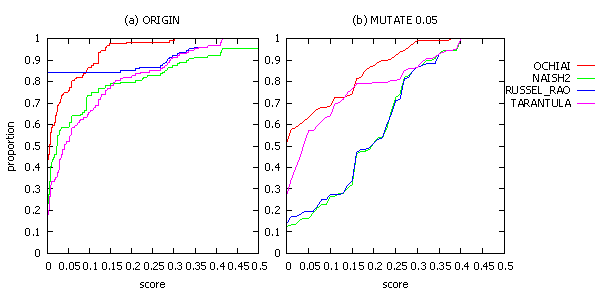
\includegraphics[width=1\linewidth]{chap02/origin_mut0_05_score}
	\caption{4种SFL算法在使用正确和错误率为0.05的测试准则时分数(score)分布情况}
	\label{fig:score-correct-0.05}
\end{figure}

\begin{figure*}
	\centering
	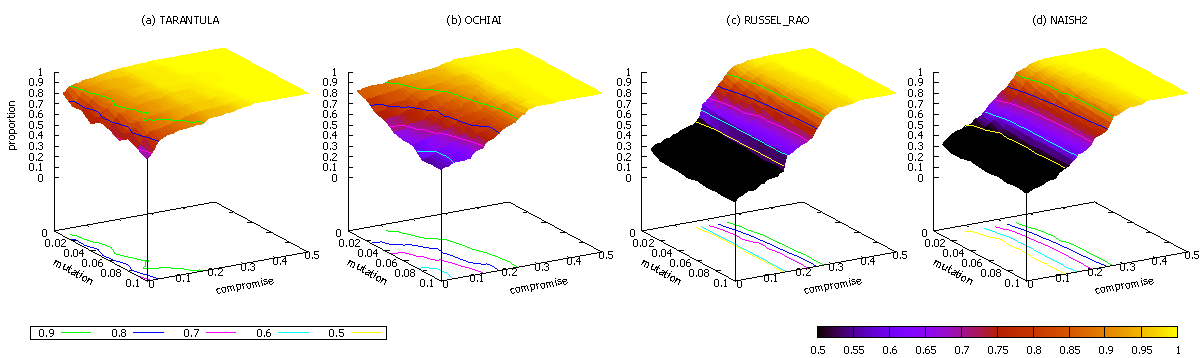
\includegraphics[width=1\linewidth]{chap02/compr}
	\caption{4中SFL算法在测试准则错误率从0.01到0.1之间是精度损耗分布情况}
	\label{fig:compr}
\end{figure*}
\section{测试Oracle纠错算法}
修正测试准则的错误判断具有一定的难度。首先,测试准则的设计初衷是检查和判断程序的正确性,而不是作为被程序检查的对象。换言之,没有其他的标准可以用来检查测试准则的正确性。考虑到测试准则最初是开发人员根据自己对程序行为的理解建立的,一种可能的解决办法是人工进行多次检查。然而,检查测试准则可能与建立一样耗时耗力。哪怕我们愿意接受这些成本,考虑到测试准则中的错误本身很难发现,重新检查一遍也未必能够清理掉这些错误。

幸运的是,在大多数情况下,测试准则中的错误可能只占很少的比例。如果利用绝大多数测试准则的正确判断,我们或许可以在某种程度上预测程序的行为,并判断程序是否应该通过某些测试用例。

受基于覆盖率的测试集压缩领域工作\cite{wong1995effect}\cite{wong1999test}的启发,我们观察到执行路径相似的测试用例通常有相似的测试结果,即这些测试用例通常是同时通过或同时不通过。研究者称,如果在保持测试过程中的基本块覆盖率(Block coverage)不变的前提下,大幅缩减测试集的规模不会对错误定位的准确度造成明显的影响。换言之,测试集中具有相似执行路径的测试用例,如果它们的基本块覆盖情况相同,通常也会有相同的测试结果(通过或不通过)。基于这一观察,本文提出利用测试用例对程序代码行的覆盖情况识别和修改测试准则中的错误。

\begin{algorithm}
	\caption{Correct the test oracle}
	\label{alg: debugMain}
	\begin{algorithmic}[1]
		\renewcommand{\algorithmicrequire}{\textbf{Input:}}
		\renewcommand\algorithmicensure {\textbf{Output:} }
		\REQUIRE $P$, $O(T)$, $n$, $thres$
		\ENSURE $O'(T)$
		\FOR {each $t_i \in T$}
		\STATE Record $Tr(P(t_i))$;
		\ENDFOR
		\FOR {each $t_i \in T$}
		\STATE Find $T_i = \{t_{i1}, t_{i2}, \ldots, t_{in}\} \subset T$ nearest to $t_i$;
		\STATE $Suspicion(t_i)$ = vote ($T_i$);
		\IF {$Suspition(t_i) > thres$}
		\STATE $O'(t_i) = \neg O(t_i)$;
		\ELSE
		\STATE $O'(t_i) = O(t_i)$;
		\ENDIF
		\ENDFOR
		\RETURN $O'(T)$;
		
	\end{algorithmic}
\end{algorithm}

算法\ref{alg: debugMain}描述了测试准则错误修正的方法框架。其输入包括程序$P$,测试集$T$及其对应的测试准则$O(T)$,投票测试用例数$n$以及“可疑值阈值”$thres$。其输出是修正后的测试准则$O'(T)$。算法分为两个步骤。步骤一,执行所有的测试用例$t_i \in T$,记录程序$P$执行测试用例$t_i$的运行路径$Tr(P(t_i))$。步骤二,首先,对所有的测试用例$t_i$,找到与之距离最近,即最相似的$n$个测试用例构成集合$T_i = \{t_{i1}, t_{i2}, \ldots, t_{in}\}$。接着,我们设计一种投票策略,让$T_i$中的测试用例的测试结果决定$t_i$的测试结果是否应该通过或不通过。投票策略的输入是$t_i$和$T_i$,输出则是一个量化的可疑值$Suspicion$,表示测试准则对$t_i$的测试结果判断$O(t_i)$出错的概率。如果$T_i$中的测试用例投票认为$t_i$的测试结果更可能是“通过”,但测试准则判断其结果为“不通过”,并且$Suspicion(t_i)$超过了预设的阈值$thres$,那么算法将判断结果取反,修改为“通过”,并记录下作为输出的$O'$对$t_i$的判断结果。

上述算法框架结构比较简单,但具体实现时仍有以下问题需要解决:
\begin{itemize}
	\item 算法的第一步需要记录测试用例的执行路径。由于已有许多成熟工具能够辅助获取执行路径(如\texttt{gcov}等),本文对这一步骤不做详细讨论。
	\item 算法的第5行在计算$T_i$时要求我们对测试用例之间的相似度做出定义,即需要定义一种依据执行路径量化测试用例之间相似性的度量公式。
	\item 算法第5行要求我们确定集合$T_i$的规模$n$的合理取值。
	\item 算法第6行要求设计一种计算测试准则判断结果可疑值$Suspicion$的策略,称为投票策略。
	\item 算法的第7行要求我们给出$thres$的合理取值。
\end{itemize}
以上问题的解决方案将影响到算法整体的有效性、时间和空间复杂度。以下我们将分节讨论这些问题。

\subsection{相似性度量}

测试用例相似性度量公式需要尽量将相似的测试用例聚集在一起,并将相异的测试用例尽量分离。
令${tr}_i = \{i_0, i_1, \ldots, i_{n_i}\}$表示测试用例$t_i$覆盖的代码行,称为$t_i$的测试轨迹集合(trace set)。量化两个集合$A$与$B$相似性的一种常用度量是$\frac{|A \cap B|}{|A \cup B|}$,受此启发,我们可以定义两个测试用例的相似度为其测试轨迹集合的相似度,即
$$
Sim(t_i, t_j) = Sim({tr}_i, {tr}_j) =\frac{|{tr}_i \cap {tr}_j|}{|{tr}_i \cup {tr}_j|}
$$

对以上公式的直观理解是,两个测试用例所共同覆盖的代码行越多越相似。但是,实际程序执行过程中,常常有很多代码行被所有测试用例都执行。例如,单元测试中的初始化代码负责构造被测单元的实例对象,在每个测试方法执行前都需运行。这部分运行路径所占比例过大将导致事实上并不相似的测试路径在上述度量上相似。事实上,被所有测试方法均覆盖的代码行不具有区分度,而被越少的测试方法覆盖的代码行越具有代表意义。因此,在依据上述公式度量两个测试用例相似度时,应为相应测试轨迹集合中的代码行赋予一定的权重。

赋权公式的设计参考了$tf-idf$\cite{wiki:tf-idf}。$Tf-idf$是\textit{term frequency - inverse document frequency}的简称,最初用于量化一个单词对一个词汇集合(corpus collection),或称为文档(document)的代表性。令$D$表示一个文档集合,$d \in D$是集合中的一个文档,$t$表示$D$中的一个词汇。词频(\textit{Term frequency}) $tf(t, d)$表示$t$在文档$d$中出现的次数。倒排词频(\textit{Inverse document frequency})度量$t$在文档集合$D$中出现的频率,定义为
$$
idf(t, D) = \log{\frac{|D|}{|\{d| d \in D \wedge t \in d\}|}}
$$

基于此,对于文档$d \in D$,$t$对$d$的权重定义为
$$tfidf(t, d, D) = tf(t, d) \times idf(t, D)
$$

回到对测试用例相似性的度量,我们可以将每个代码行看做为一个单词$t$,将每个测试路径集合看做文档$d$,将所有测试路径集合看做文档集合$D$。在此模型下,对$t_i \in T$, $i_p \in tr_i$, $tf(i_p, t_i) = 1$,因此
$$
tfidf(i_p, t_i, T) = idf(i_p, T) = \log{\frac{|T|}{|\{t_l|t_l \in T \wedge i_p \in t_l\}|}}
$$

将权重与集合相似度公式相结合,最终我们定义两个测试用例$t_i$和$t_j$之间的相似度为
$$
Sim (t_i, t_j) = \frac{\sum_{i_p \in {tr}_i \cap {tr}_j}^{} tfidf(i_p, t_i, T)}{\sum_{i_p \in {tr}_i \cup {tr}_j}^{} tfidf(i_p, t_i, T)}
$$
注意,此处$tfidf(i_p, t_i, T)$实际上$t_i$无关,因此$Sim(t_i, t_j) = Sim(t_j, t_i)$,即公式对$t_i,t_j$满足交换律。此外,${tr}_i \cap {tr}_j \subset {tr}_i \cup {tr}_j$,因此$0 \le Sim(t_i, t_j) \le 1$恒成立。

\subsection{投票策略}
对测试用例$t_i$,我们计算其与所有其他测试用例的相似度,并选出其中与之相似度最高的$n$个测试用例构成投票组。购票组中测试用例的测试结果将用于决定$t_i$的测试结果是否正确。设$T_{i, p} = \{t_{iq} | O(t_{iq}) = \mathcal{P}, t_{iq}\in T_i\}$, $T_{i, f} = \{t_{iq} | O(t_{iq}) = \mathcal{F}, t_{iq}\in T_i\}$,分别表示投票组中被实际测试准则$O$判别为“通过”和“不通过”的测试用例集合。定义$Vote_{ip} = \sum_{t_{iq} \in T_{i, p}} Sim(t_i, t_{iq})$,$Vote_{if} = \sum_{t_{iq} \in T_{i, f}} Sim(t_i, t_{iq})$,分别表示投票为“通过”和“不通过”的计票数,则$t_i$的测试结果可疑值Suspicion按如下公式计算。
$$
Suspicion(t_i) = \left\{
\begin{array}{lr}
\frac {Vote_{ip}}{Vote_{ip} + Vote_{if}}     & if \ O(t_i) = \mathcal{F} \\
\frac {Vote_{if}}{Vote_{ip} + Vote_{if}}     & if \ O(t_i) = \mathcal{P}
\end{array}
\right.
$$

\subsection{参数设置}
\label{subsection: param}

算法\ref{alg: debugMain}涉及两个重要的参数,其一是投票组中的测试用例数$n$,二是可疑度阈值$thres$。这两个参数都是预设的常数,因此其值应科学选取。从直观上分析,若$n$太小,如$n = 2$,那么很可能投票组中的两个测试用例的测试结果也有错误,那么投票结果也是不可信的。而如果$n$过大,则投票组中将很可能包含许多与所关心的测试用例并不相似的测试用例,其投票结果同样不可靠。类似的,若参数$thres$设置的过高,那么测试准则的判断错误将可能被漏掉。相反,若$thres$太低,则很多实际正确的测试结果会被误认为错误。

理想的参数配置使算法能够尽量保留正确的测试结果,同时识别出错误的测试结果,也即应当降低假阳性(false positive,简称FP)和假阴性(false negative,简称FN)的数目。设置参数的困难在于,在算法的实际应用中,我们预先并没有一个完全正确的测试准则作为参考,自然也不能对FP和FN准确计数。换言之,哪怕将所有的$n$和$thres$的组合遍历一次,我们仍然无法选出哪一组参数的设置是最合理的。

%TODO: try modify this paragraph.. it just doesn't feel good..
事实上,从给定所期望的FP和FN出发寻找恰当的$n$和$thres$是比较困难的,但从相反的方向分析$n$和$thres$的不同取值对FP和FN的影响则是可行的。本节我们分析FP、FN与$n$、$thres$的概率关系。分析基于以下两个假设:

\textit{假设1} : $\forall t_{iq}\in T_i \cup \{t_i\}$, $O_c(t_{iq}) \in \{\mathcal{P}, \mathcal{F}\}$  $i.i.d.$.

\textit{解释}:一个测试用例的运行结果与其他测试的运行结果不相关,因此每个$t_{iq}\in T_i \cup \{t_i\}$, $O_c(t_{iq})$都是独立的。另外,由$T_i$的生成方式可知,任一$t_{iq}\in T_i$与$t_i$均足够相似,因此我们可以合理的假设这些测试用例的测试结果的概率分布也是相同的。

\textit{假设2} : $\forall t_{iq_1}$, $t_{iq_2} \in T_i \cup \{t_i\}$, $iq_1 \ne iq_2$,
$\mathbf{P}(O_c(t_{iq_1}) = O_c(t_{iq_2})) = {sim}_i\  (常数)$

\textit{解释}: 由于$O_c(t_{iq}) \in \{\mathcal{P}, \mathcal{F}\}\ i.i.d.$, 显然存在常数$\alpha_i \in [0,1]$满足$\forall t_{iq_1}$, $t_{iq_2} \in T_i \cup \{t_i\}$, $iq_1 \ne iq_2$, $\mathbf{P}(O_c(t_{iq_1}) = O_c(t_{iq_2})) = \alpha_i$。根据上文中的观察,测试用例越相似,具有相同结果的概率就越高,因此我们可以用${sim}_i$估计$\alpha_i$。

在以上两条假设下,我们可以得到以下结果:对任意$t_i \in T$,经算法\ref{alg: debugMain}计算得到的$O_c(t_i)$是FN的概率是	
\begin{equation}
\label{equ: fn single}
\mathbf{P}(fn(t_i))	\approx r \sum_{w = 0}^{\hat{n}}{\mathrm{C}_n^w{\phi_i^w (1-\phi_i)^{(n-w)}}}
\end{equation}

而$O_c(t_i)$是FP的概率是
\begin{equation}
\label{equ: fp single}
\mathbf{P}(fp(t_i)) \approx (1 - r) \sum_{w = \hat{n} + 1}^{n} \mathrm{C}_n^w{(1 - \phi_i)^w} \phi_i^{(n-w)}
\end{equation}

其中$\phi_i = \beta_{i2} + r - 2 \beta_{i2} r$,$\beta_{i2} = \frac{1 + \sqrt{2 sim_i - 1}}{2}$,$sim_i$是$T_i$中所有测试用例与$t_i$相似度的平均值,$\hat{n} = \lfloor n \times thres \rfloor$,$r$是测试准则的错误率。

公式\ref{equ: fn single}和\ref{equ: fp single}的详细推导过程请参见附录\ref{cha:proof}。

上述公式可以指导$n$和$thres$的取值决策过程。决策过程的第一步是分析$\phi_i$的取值情况。$\phi_i$是$r$和$sim_i$的函数,图\ref{fig:phi}展示了三者之间的量化关系。
\begin{figure}
	\centering
	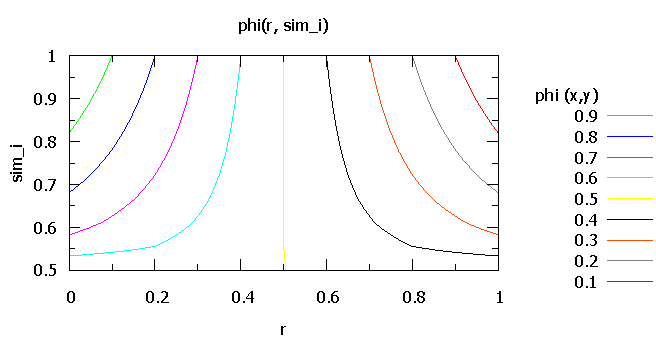
\includegraphics[width=0.7\linewidth]{chap02/phi}
	\caption{$\phi_i$随$r$和${sim}_i$的变化情况}
	\label{fig:phi}
\end{figure}
如图所示,$0 < \phi_i < 1$。由于我们假定测试准则的大部分判断是正确的,即$r > 0.5$,并且在这一范围下,$\phi_i > 0.5$,因此显然$\mathbf{P}(fn(t_i))$随$\hat{n}$的增加而剧烈增加,$\mathbf{P}(fp(t_i))$随$\hat{n}$的增加而剧烈减少。
合理的参数取值应当使FN和FP的比例同时尽可能低。直观上似乎应使$thres = 0.5$,这样FP和FN都不会太高,而量化分析的结果也确实如此。表\ref{tab:calculate fp fn}列出了$P(fn(t_i))/r$和$P(fp(t_i))/(1 - r)$两个算式在$n = 3, 4, 5$,$\hat{n} = 1,\cdots, 4$及$\phi_i = 0.7, 0.8, 0.9$所有组合下的取值。表格中标红的参数组合是在确定$n$的取值下我们选出的最优参数组合。选择的理由有两个,首先$r$相对较小,一个较大的$P(fn(t_i))/r$与之相乘时计算结果也不会很大,但是一个较大的$P(fp(t_i))/(1 - r)$与$(1-r)$相乘则计算结果也会较大,因此在$n = 4$时我们选择$\hat{n} = 2$。第二,实验结果表明FP的存在对SFL算法精度的负面影响更加明显,使$\hat{n}$与$n$距离稍远可以带来更好的错误定位精度,因此在$n = 5$时我们选择$\hat{n} = 2$。
\begin{landscape}
	
\begin{table}
	\centering
	\caption{$fp(t_i)$和$fn(t_i)$的概率随$\phi_i$,$n$和$\hat{n}$的变化}
	\label{tab:calculate fp fn}
	\begin{tabular}{c|c|cc|ccc|cccc}
		\hline
		\multicolumn{2}{l}{$n$} \vline& \multicolumn{2}{c}{3}  \vline & \multicolumn{3}{c}{4} \vline & \multicolumn{4}{c}{5} \\ \hline \multicolumn{2}{l}{$\hat{n}$} \vline &   $1$    &   $2$    &   $1$    &   $2$    &   $3$    &   $1$    &   $2$    &   $3$    &   $4$    \\ \hline
		$\phi_i = 0.7$        & $\mathbf{P}(fn(t_i)) / r$ & \color{red}$0.2160$ & $0.6570$ &$0.0837$ &  \color{red} $0.3483$ & $0.7599$ & $0.0307$ & \color{red}$0.1630$ & $0.4717$ & $0.8319$ \\  \cline{2-11}
		& $\mathbf{P}(fp(t_i)) / (1 - r)$ & \color{red}$0.2160$ & $0.0270$ & $0.3483$ & \color{red}$0.0837$ & $0.0081$ & $0.4718$ & \color{red}$0.1630$ & $0.0308$ & $0.0024$ \\ \hline
		
		$\phi_i = 0.8$        & $\mathbf{P}(fn(t_i)) / r$ & \color{red}$0.1040$ & $0.4880$ &$0.0272$ &  \color{red}$0.1808$ & $0.5904$ & $0.0067$ & \color{red}$0.0579$ & $0.2627$ & $0.6723$ \\  \cline{2-11}
		& $\mathbf{P}(fp(t_i)) / (1 - r)$ & \color{red}$0.1040$ & $0.0080$ & $0.1808$ & \color{red}$0.0272$ & $0.0016$ & $0.2627$ & \color{red}$0.0579$ & $0.0067$ & $0.0003$ \\ \hline
		
		$\phi_i = 0.9$        & $\mathbf{P}(fn(t_i)) / r$ & \color{red}$0.0280$ & $0.2710$ & $0.0037$ & \color{red}$0.0523$ & $0.3439$ & $0.0005$ & \color{red}$0.0085$ & $0.0814$ & $0.4095$ \\  \cline{2-11}
		& $\mathbf{P}(fp(t_i)) / (1 - r)$ & \color{red}$0.0280$ & $0.0010$ & $0.0523$ & \color{red}$0.0037$ & $0.0001$ & $0.0814$ & \color{red}$0.0085$ & $0.0005$ & $0.0000$ \\ \hline
		
		
	\end{tabular}
	
\end{table}
\end{landscape}
表\ref{tab:calculate fp fn}中给出的参数选择方案仅考虑了如何针对某一个特定$t_i$降低$P(fn(t_i))$和$P(fp(t_i))$。若要降低测试集整体的FP和FN数目则需要知道所有测试用例的$\phi_i$。但$\phi_i$是$n$的函数,因此在确定$n$前我们无法得知$\phi_i$的值。打破这一循环的关键在于,从表\ref{tab:calculate fp fn}中的数据我们可以得到这样的结论,当给定某一$n$时,$\hat{n}$的最佳取值与$\phi_i$的变化无关。因此,尽管测试用例的${sim}_i$各不相同,一旦$n$确定后,我们不需要对每个测试用例单独设置一个$thres$值。换句话说,尽管我们无法将所有测试用例的$P(fn(t_i))$和$P(fp(t_i))$逐一计算出,我们仍然可以为所有测试用例统一选择一个最优的$thres$值。

上述分析将问题简化为选择一个合理的$n$。根据表\ref{tab:calculate fp fn}中的数据,$\phi_i$值越大,$P(fn(t_i))$和$P(fp(t_i))$的值越小。因此,如果$\phi_i$较小,则$n$可相应的取一个较大的值用以保证算法的正确率。但是当$\phi_i > 0.8$时,取$n = 4$算法的正确率已经比较好。在实际应用中,如果有先验知识可以用来估计$\phi_i$,那么可以使用表\ref{tab:calculate fp fn}作为确定$n$取值的参考。如果没有先验知识,可以按照如下步骤选择$n$:(1)执行所有测试用例,获取测试路径集合,(2)在测试集上随机选取一个子集作为样本,为子集中所有测试用例找到全集中的$10$个距离最近的邻居,(3)计算这些邻居间的相似度。根据这一数据,我们可以估计$sim_i$的值,也能够迅速了解每个测试用例周围的邻居的数目。如果$sim_i$很低,或者邻居很少,可能我们需要为测试集补充新的测试用例。反之,如果$sim_i$足够高,邻居也比较充足,那么只要$r$不太大,算法最终的正确率应当仍有保证。不管怎样,即使是在需要补充新的测试用例的情况下,由于测试准则本身是有错的需要修改,我们并没有为测试人员增加额外工作量。

\subsection{时间与空间复杂度分析}

算法\ref{alg: debugMain}包含两个阶段,即测试轨迹获取和测试准则调试。第一阶段的时间和空间复杂度取决于所使用的的轨迹获取工具(例如\texttt{gcov}),但存储所有测试路径集合需要的空间复杂度为$O(|T|N)$。在第二阶段,首先我们需要计算每一行代码的权重,即$tf-idf$值,这将带来$O(|T|N)$的时间复杂度,但并不需要申请新的空间。接着我们计算任意两个测试用例之间的“相似度”,这一操作的时间复杂度为$({|T|}^2 O(sim))$,其中$O(sim)$是计算给定两个测试用例之间的相似度的时间复杂度,空间复杂度是$O({|T|}^2)$。在本文的实现中,$O(sim) = O(N)$。
算法的下一步骤是计算每个测试用例$t_i$的邻居集合$T_i$,这一步骤最简单的实现需要$O({|T|}^2 n)$的时间复杂度和$O(|T| n)$的空间复杂度。最后,算法计算每个测试用例的“可疑值”,时间复杂度是$O(|T| O(Sus))$,其中$O(Sus)$是计算一个给定测试用例可疑值的时间复杂度,空间复杂度最多为$O(|T|)$。在本文实现中,$O(Sus) = O(n)$。因此,算法的总时间复杂度是$\max\{O({|T|}^2 O(sim)), O({|T|}^2 n), O(|T| O(Sus))\} = O({|T|}^2 N)$,总空间复杂度是$O(|T| N)$。这一结果说明,时间复杂度随程序规模的增加而线性增加,随测试集规模的增加而平方增加,空间复杂度随程序规模和测试规模的增加而线性增加。

\section{实验结果及分析}
\label{sec: experiments}
算法\ref{alg: debugMain}性能需两个方面评价,一是纠错后的测试准则的判断结果正确性有多大程度的提升,二是使用纠错后的测试结果应用SFL算法的错误定位精度有多大程度的提升。本节将以两个实验及其实验数据分别对这两个问题做出回答。

\subsection{修复测试准则错误}
\label{subsection: repair test oracle}
实验一的目的是评价纠错后的测试准则的正确率,并与纠错前的测试准则作对比。在本实验中,我们使用西门子测试集作为对象程序,这是由于该测试集中的每个程序均含有足够多的测试变体,从而能够保证测试结果的统计显著性。与第三节中的实验相似,我们首先生成正确的测试准则,并将测试准则的判断按照概率$mr$随机改变,其中$mr \in [0.01, 0.1]$。

算法\ref{alg: debugMain}在具体实现时需要确定两个参数的值,即投票集合大小$n$和纠错阈值$thres$。遵照上节中的参数选择方法,我们首先随机选取了一部分测试用例作为样本,结果表明几乎所有的测试用例都有至少10个相似值超过0.9的邻居。完整的实验数据表明,事实上整个测试集中约有超过95\%的测试用例拥有相同数量的邻居。参考表\ref{tab:calculate fp fn}中的数据,我们认为$n=4$已经足够获得较好的性能。另一方面,在$thres$的设置上,根据前文的分析,只要$2 < \hat{n} < 3$就可以得到一个较好的结果。最终在所有的程序上我们都使用了$thres = 0.58$这一参数值。

将$n = 4$和$thres = 0.58$带入到算法框架中,我们在待修改的测试准则上运行了调试算法,并将输出结果与输入结果对比。按照\cite{Steimann:2013:TVV:2483760.2483767}中的要求,为获得稳定可靠的结果,我们将实验重复了五次。实验结果的观察指标共三个,包括(1)召回率(recall),表示算法发现测试准则错误的能力,(2)精度(precision),表示算法保留测试准则正确判断的能力,(3)F1指数(f1 measure),表示前两个指标的综合成绩。

图\ref{fig:mut_rec_prec_cropped}展现了三个指标在所有程序变体和不同错误率下的分布情况。其中,给定召回率$rec$、错误率$mr$,纵坐标比率$p(rec, mr)$的含义是,在错误率$mr$时,所有输出测试准则的召回率不低于$rec$的测试用例占测试集的比例$mr$。 对精度$pre$和F1指数$f1$,$p(pre, mr)$和$p(f1, mr)$也有类似定义。
\begin{figure}
	\centering
	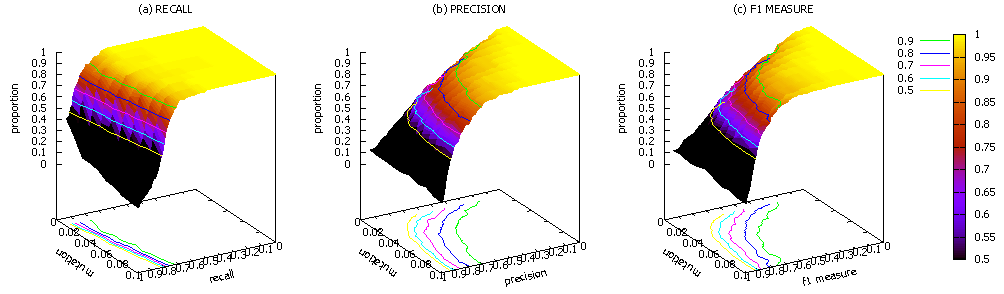
\includegraphics[width=1\linewidth]{chap02/mut_rec_prec}
	\caption{$mr$在$[0.01,0.1)$时召回率、准确率和f1指数分布情况}
	\label{fig:mut_rec_prec_cropped}
\end{figure}
如图所示,平均来看算法在超过90\%的程序变体上达到了85\%的召回率,也即超过85\%的测试准则错误被成功发现。另一方面,算法在不同错误率的测试准则上达到的精度也各不相同。当$mr$取中位数$0.05$时,在超过80\%的程序变体上算法的精度达到了75\%,即算法所识别出的测试准则错误中超过75\%的确是错误。当$mr$增长到$0.1$时,算法精度上升到80\%。这一趋势也在F1指数的图像上显示出来,当$mr$趋向1时,由于召回率接近1,F1指数的图像与精度类似。

观察在x-y平面上的等高线投影可以发现一个有趣的现象。首先,当$mr$低于$0.02$时,在50\%的测试用例上,算法识别出的错误中超过20\%是FP,在30\%的测试用例上,FP比率超过了40\%。另一方面,召回率在约80\%左右的程序变体上超过了90\%,可见实验数据与直觉完全相符,当召回率很高时,FN较低,FP较高,精度也较低。
%More importantly, this also substantiates our theoretical analysis of the probability of false positive and false negative. Referring to Table \ref{tab:calculate fp fn}, suppose $\phi_i \approx 0.9$, then theoretically $\frac{\mathbf{P}(fn(t_i))}{r} \approx 0.0523$ and $\frac{\mathbf{P}(fn(t_i))}{1 - r} \approx 0.0037$. If $r = mr \in [0.01, 0.02]$, then $\mathbf{P}(fn(t_i)) \in [0.0005, 0.0010]$ and $\mathbf{P}(fp(t_i)) \approx 0.0037$. On the other side, let $tp$ be the true positive rate, then $rec = \frac{tp}{tp + fn}$, $pre = \frac{tp}{tp + fp}$. Reading from the figure, average recall $rec \approx 0.9$, average precision $pre \in [0.7, 0.8]$. Remember $tp + fn = mr$, then we can calculate the in our experiments $fp \in [0.001, 0.002]$ and $fp \in [0.0023, 0.0075]$. Consider the imprecise estimation of $\phi_i$, it is reasonable to claim that the experimental result and theoretical probabilistic analysis match.
其次在第四节的理论分析中,我们得出结论当$thres$和$n$保持不变时,$\mathbf{P}(fn(t_i))/r$和$\mathbf{P}(fp(t_i))/(1-r)$均基本保持不变,因此当$r$升高时,$\mathbf{P}(fn(t_i))$上升而$\mathbf{P}(fp(t_i))$下降。实验数据也验证了这一结论,当$mr$升高时,召回率略微下降,但精度显著上升。


\subsection{SFL算法精度恢复}

实验二的目的是研究SFL算法的定位精度在使用纠错后的测试准则判断的测试结果时会恢复到怎样的程度。实验用的对象程序包括西门子测试集以及代码规模超过13,000行的程序\texttt{grep}。

\subsubsection{西门子测试集上的实验结果}
作为基准参考,我们首先使用错误的测试准则,统计四种SFL算法在所有西门子测试集中的程序变体上错误定位的精度。接着使用算法\ref{alg: debugMain}对测试准则纠错。最终重新统计四种SFL算法错误定位的精度,并与之前的精度进行对比。与第\ref{sec: error impact}节中的数据统计方式保持一致,错误定位精度被量化为公式\ref{equ: score}定义的分数(score)。实验重复了5次,实验结果如图\ref{fig: perfomance_improvement}所示。

图\ref{fig: mutScore}和图\ref{fig: autoScore}展示了测试准则纠错前后SFL的精度的对比情况。给定错误率$mr$和分数$s_x$,图中的纵坐标比率(proportion)$p(mr, s_x)$表示当测试准则的错误率为$mr$时,所有错误定位精度高于$s_x$的程序变体在测试集中所占的比例。

直观的看,图\ref{fig: autoScore}中四种算法对应图像的曲面都比图\ref{fig: mutScore}中对应的曲面明显提高,这意味着SFL算法的定位精度也有了明显提升。具体而言,在使用错误的测试准则时,Russel\&Rao在约20\%的程序变体上定位精度分数为$0$(即错误代码行被排在第一位),而当使用纠错后的测试准则时,这一比例扩大到超过50\%。对Ochiai,这一比例从少于60\%扩大到超过70\%。在第三节的实验中,Tarantula表现出较好的容错性,但这一比例从25\%扩大到40\%,说明其定位精度也有了较大的提高。

为了更清晰的观察图\ref{fig: autoScore}和图\ref{fig: mutScore}之间的区别,我们绘制了另外两组图片来展示SFL算法精度的绝对(图\ref{fig: mut-absImp})和相对(图\ref{fig: mut-relImp})提高。准确起见,除在第\ref{subsection: compr result}小节定义的$s_0(v_i, \omega_j)$和$s_r(v_i, \omega_j)$之外,我们定义$s_d(v_i, \omega_j)$用以表示SFL算法$\omega_j$以纠错后的测试准则判断作为输入应用于程序变体$v_i$达到的定位精度,则算法$\omega_j$在测试准则错误率为$r$应用于$v_i$时精度的绝对提高定义为
$$
\Delta_{|\cdot|}^{+}(\omega_j, v_i, r) = s_r(v_i, \omega_j) - s_d(v_i, \omega_j)
$$
相对提高定义为
$$
\Delta_{\%}^{+}(\omega_j, v_i, r) = \frac{s_d(v_i, \omega_j) - s_0(v_i, \omega_j)}{s_r(v_i, \omega_j) - s_0(v_i, \omega_j)}
$$

在这两张图中,给定$\Delta_x$和测试准则错误率$r$,纵坐标比率$p$的含义是所有在测试准则纠错前后SFL的精度提高超过了$\Delta_x$的测试用例所占比例。如图\ref{fig: mut-absImp}所示,不同算法的精度在不同程度上有所提高。例如,使用算法Russel\&Rao,在约有30\%的程序变体上算法精度提高了10\%,这意味着在实际的“生成-检验”系统实现中,搜索引擎所需检查的代码减少了10\%,搜索效率大大提升。

从图\ref{fig: mut-absImp}中的图像来看,似乎在许多程序变体上SFL的精度提高并不明显。这是因为对于大多数程序而言,哪怕是使用错误的测试准则作为输入,SFL的定位精度分值仍然在30\%以下,因此绝对提升的空间有限。但是图\ref{fig: mut-relImp}显示,对超过50\%的程序变体而言精度的相对提升幅度较大,提升最明显的是Russel\&Rao,在超过50\%的程序变体上定位精度的相对提升幅度超过了50\%。

从图\ref{fig: perfomance_improvement}中可以看出,SFL算法的定位精度在测试准则经过纠错后有了明显恢复。由于这四种算法都是研究公认的“最优”或应用最广泛的是算法,因此我们认为这一结论可以推广到SFL一族的其他算法上。

\begin{figure}
	\centering
	\begin{subfigure}{15cm}
		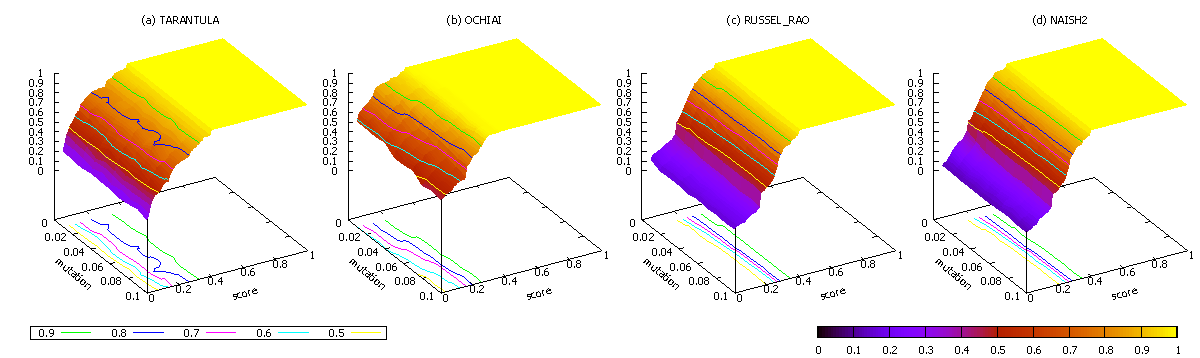
\includegraphics[width=1\linewidth]{chap02/mut_mutScore}
		\caption{Score distribution on erroneous oracle mutants}
		\label{fig: mutScore}
	\end{subfigure}%
\hspace{0.5cm}
	\begin{subfigure}{15cm}
		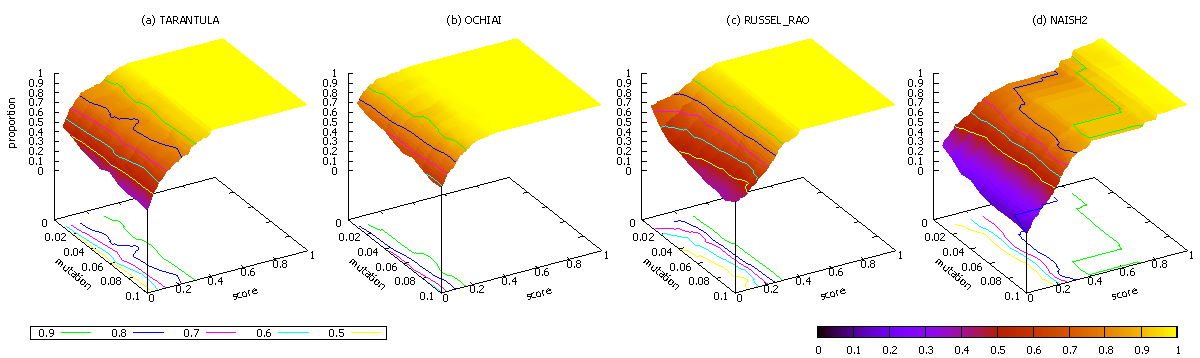
\includegraphics[width=1\linewidth]{chap02/mut_autoScore}
		\caption{Score distribution on debugged mutants}
		\label{fig: autoScore}
	\end{subfigure}%
\hspace{0.5cm}
	\begin{subfigure}{15cm}
		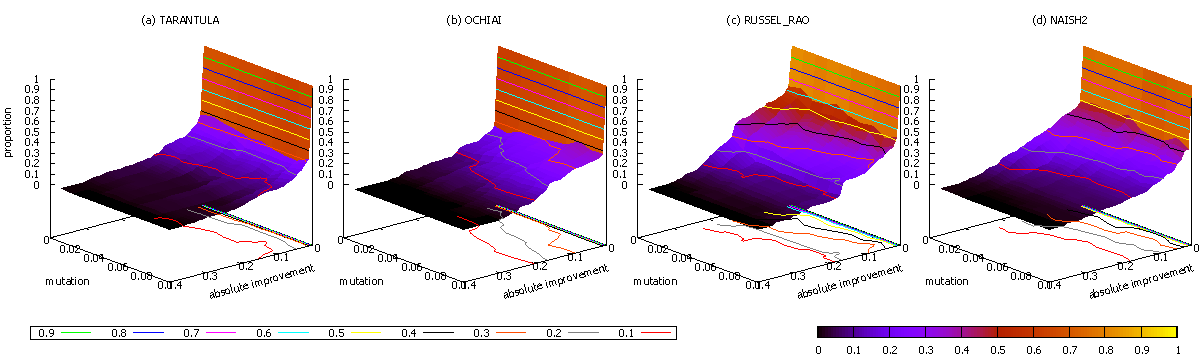
\includegraphics[width=1\linewidth]{chap02/mut_absImp}
		\caption{Distribution of absolute improvement}
		\label{fig: mut-absImp}
	\end{subfigure}%
\hspace{0.5cm}
	\begin{subfigure}{15cm}
		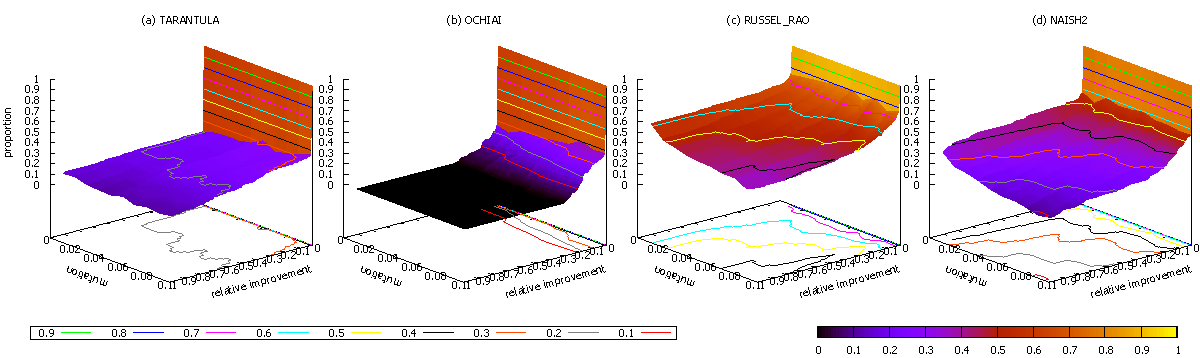
\includegraphics[width=1\linewidth]{chap02/mut_relImp}
		\caption{Distribution of relative improvement}
		\label{fig: mut-relImp}
	\end{subfigure}%
	
	\caption{4种SFL算法在修正后的测试准则下的定位精度恢复情况}
	\label{fig: perfomance_improvement}	
\end{figure}
\subsubsection{\texttt{grep}上的测试结果}

\texttt{grep}是类Unix系统中常用的字符串匹配程序,其功能是在文本文件中查找符合某一模式的字符串。SIR\cite{doESE05}提供了\texttt{grep}的5个发布版本,每个版本都包括18个有植入错误的程序变体及其相应的测试集。初步测试显示,很多程序变体中的错误无法被测试集中的测试触发,因此本节实验的程序对象将这部分程序变体移除了。特别的,版本5只有一个程序变体,但其中的错误无法被触发,因此版本5整体被移除了。表\ref{Tab: grep-info}列出了基本发行版本的基本信息。

\begin{table}
	\caption{\texttt{grep}基本信息} \label{Tab: grep-info}
	\centering
	\begin{tabular}{c|c|c|c}
		\hline 版本号 & 植入错误数 & 可检测的错误数 & 代码行数 \\ 
		\hline v1 & 18 & 2 & 12654 \\ 
		\hline v2 & 8 & 1 & 13231 \\ 
		\hline v3 & 18 & 2 & 13374 \\ 
		\hline v4 & 12 & 2 & 13360 \\ 
		\hline v5 & 1 & 0 & 13293 \\ 
		\hline
	\end{tabular} 
\end{table}

与在西门子测试集上的实验设计相同,我们首先利用未植入错误的程序版本为所有程序变体生成了正确的测试准则,接着按概率$mr\in [0.01, 0.1]$随机改变测试准则的输出获取错误的测试准则,最终比较SFL算法在错误的测试准则和纠错后的测试准则上的定位精度。实验重复了5次,图\ref{Fig: grep}展示了实验结果。

\begin{figure}
	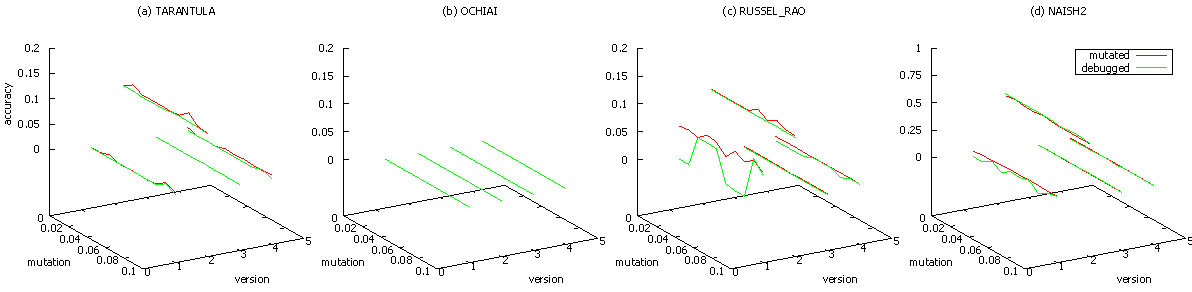
\includegraphics[width=1\linewidth]{chap02/grep}
	\caption{SFL算法在\texttt{grep}程序上使用正确与错误测试准则的精度对比}
	\label{Fig: grep}
\end{figure}

图\ref{Fig: grep}展示了在四个版本的\texttt{grep}上SFL的错误定位精度。鉴于总共只有4个版本,我们可以更清晰的看到算法\ref{alg: debugMain}对每个程序的影响。对使用同一SFL算法的每个版本的程序,红线表示当测试准则错误率在$[0.01,0.1)$上变化时定位精度的变化情况,绿线表示使用纠错后的测试准则时的定位精度。在大多数程序变体上,所有SFL算法的定位精度都有所提高。其中变化最显著的是Russel\&Rao,Ochiai的精度虽没有明显提高,但也没有降低。

值得注意的是,西门子测试集中,每个程序都有约4000个测试用例,因此算法能够很方便的利用测试用例之间的相似性达到较好的召回率和精度。与之对比,SIR为\texttt{grep}提供的测试用例集是\textit{“能够代表实际开发过程中使用的测试用例”}\cite{doESE05},所包含的测试用例只有199个,实验数据显示算法仍然取得了较好的效果。这说明算法\ref{alg: debugMain}能够应用于实际程序的真实测试集。

\section{讨论}
在第\ref{sec: experiments}节的实验二中,我们观察到随着测试准则错误率的上升,SFL算法在纠错后的测试准则上的精度提升有小幅度的下降。这一趋势恰好与召回率随测试准则错误率的变化趋势相同,那么召回率与SFL算法的精度提升幅度之间是否有不通过测试准则错误率的直接关系呢?考虑到Russel\&Rao的精度提升最明显,我们计算了绝对精度提高和相对精度提高在不同召回率上的分布情况,图像如图\ref{fig:rec_abs_relImp}所示。

在图\ref{fig:rec_abs_relImp}中,我们画出了当绝对(相对)精度提升在$0$和$1$之间取值时,达到不同召回率的程序变体所占的比率。尽管曲面有许多皱褶,我们仍然可以从$x-y$平面的等高线投影上看到精度提升随着召回率的升高而升高的大致趋势。

从这一趋势可以得出的一个直接结论是,与测试准则的错误率无关,一般而言较高的召回率也对应着较大的SFL的精度提高幅度。因此,只要调整算法中的参数获得较好的召回率,本节所提出的方法也能够在测试准则错误率超过$0.1$(本实验中的上限)场景下应用。

%TODO:??
此外,我们还可以推断出测试准则的哪一类错误,即“假通过”或“假失败”,对SFL算法的精度影响更大?这一问题的重要性在于,在实际的软件开发过程中,尽量避免测试准则错误总是比使用SFL定位错误更加经济。分析实验数据我们发现,对于西门子测试集中的绝大多数程序变体,大约有5\%的测试用例能够触发程序中的错误,这导致大多数的测试准则错误是“假失败”,而“假通过”很少发生。当召回率较高时,几乎所有的测试准则错误都会被纠正过来,这大幅减少了“假失败”的数量,但对“假成功”影响较小。这样一来,召回率实际上可以被当做纠错后的测试准则其中所包含的错误类型分布的观察指标,即较高的召回率通常意味着较少的“假失败”和较多的“假成功”。由图\ref{fig:rec_abs_relImp}中的趋势可以看出,较少的“假失败”也和更明显的SFL定位精度提高同时出现。因此我们可以得出结论,“假失败”的确对SFL定位精度的影响更严重,在实际开发过程中应当尤其注意避免。

\begin{figure}
	\centering
	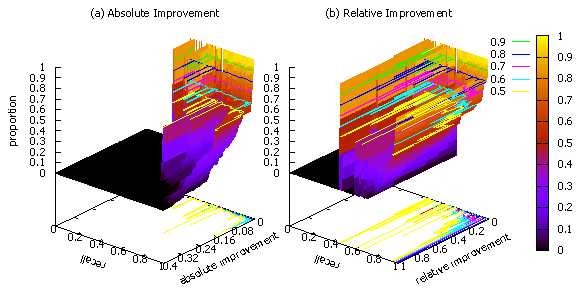
\includegraphics[width=0.8\linewidth]{chap02/rec_abs_relImp}
	\caption{绝对与相对精度提升与召回率的关系}
	\label{fig:rec_abs_relImp}
\end{figure}

%\section{Threats to Validity}

本章中第三节与第五节中的实验均属于经验研究,其结论的正确性可能受到多种因素的影响。我们参考\cite{Steimann:2013:TVV:2483760.2483767}中总结出的几个方面作如下分析。

第一个因素是被研究程序对象是否具有代表性。在第\ref{sec: error impact}节的实验研究中,研究对象是西门子测试集。西门子测试集的一个问题是其中包含的被测程序的规模都比较小,因此实验得出的结论可能无法完全准确的反映测试准则错误对大型程序的影响。但是这并不影响我们得出的测试准则错误会对错误定位精度产生影响这一结论。在第\ref{sec: experiments}节,我们使用超过13,000行代码的真实程序\texttt{grep}作为研究对象,并在第\ref{sec: experiments}节证明错误定位准确度由于修正了测试准则而提高,由此我们认为本章所提出的算法可以应用于一般规模的真实程序。

第二个因素是被研究程序的错误种类是否全面,即是否同时考虑了单一错误及多种错误两种情况。本章中的实验对象均是单一错误对象,但是在第\ref{subsection: compr result}小节的分析中我们指出,许多单一错误对程序的实际影响可以模拟多处错误,例如一个错误的常量定义可能导致程序中所有使用这一常量的地方都是错误的。实验中我们也刻意保留了这些错误,使实验结果能够更贴近实际应用。

第三个因素是采样规模,即被研究程序对象的数量。\cite{Steimann:2013:TVV:2483760.2483767}中强调需要至少300个被测程序实验的统计结果才能稳定,因此我们进行了5次重复实验来减少实验结果的随机性。

最后\cite{Steimann:2013:TVV:2483760.2483767}中提到的一个因素是测试集的质量,即测试集的规模和覆盖率。西门子测试集为每个被测程序都提供了充足的测试用例,测试集的覆盖率也足够好。程序\texttt{grep}只包含了199个测试用例,但由于我们希望实验结果能够“代表实际开发过程中的程序”,\cite{doESE05},因此没有对测试集作进一步的扩充。综合两种类型的测试集,我们认为本章的实验结果能够充分支持实验结论。


\section{本章小结}

在本章中,我们首先提出测试准则错误会对“生成-检验”系统中的第一步“错误定位”造成负面影响。为了确认这一影响,我们在西门子测试集上进行试验,测试SFL算法的定位精度受测试准则错误的影响。与使用完全正确的测试准则相比,实验数据使用有错的测试准则会使得不同的SFL算法的定位精度有不同程度的下降。因此得出结论,应在错误定位这一环节前修正测试准则错误。

基于一个简单的假设,即“覆盖相似代码行的测试用例通常同时通过或不通过”,我们提出了基于代码行覆盖情况度量测试用例间相似度的方法,并在此基础上提出利用邻居测试用例投票估计测试准则对测试结果的判断出错的可疑程度,并将可疑程度超过某一阈值的测试准则判断翻转,作为测试准则纠错的结果。实验显示,这一算法能够识别出大多数的测试准则判断错误。更进一步的,我们在西门子测试集和\texttt{grep}上比较了4种SFL算法在使用纠错前和纠错后的测试准则判断时的定位精度。实验结果显示,4中SFL算法的定位精度均有恢复。最后,通过对实验数据的进一步分析,我们得出结论,本章算法可以适用于测试准则的错误率超过实验中所设的上限$0.1$的情况。